\chapter{Struktur und Aufbau des Programs}

%
%
%
\section*{Layout}
\label{sec:layout}

Das Seitenlayout ist durch ein einfaches Gridlayout definiert und beinhaltet folgende Bereiche
\begin{description}
  \item[Kopfbereich] Hier steht der Name der Anwendung. Dieser Bereich änder sich nicht in der gesamten Anwendung.
  \item[Inhaltsbereich] Hauptinhalte jeder Unterseite wird hier dargestellt.
  \item[Schnellnavi] Die Schnellnavigation erlaubt einen Schnellzugriff auf wichtige Bereiche der Anwendung. Die Navigationsknüpfe sind durch Symbole (Icons) repräsentiert. Die navigationsleiste ist rechts ausgerichtet. Und enthält folgende Navigationsknöpfe:
  \begin{description}
    \item[Modulseite] \texttt{module-page-icon.png} Führt zur Hauptseite des aktuellen Moduls. 
    \item[Modulseite] \texttt{main-page-icon.png} Führt immer zur Hauptseite. 
    \item[Login/Profil] \texttt{login-icon.png / profile-icon.png} Führt zur Login- bzw. zur Profilseite. 
    \item[Hilfe] \texttt{help-icon.png} Öffnet Overlay mit Hilfe zur aktuellen Seite. 
  \end{description}
  
  \item[Wo bin ich] Dreizeiliger Text mit Angabe der aktuellen Position in der Anwendung. Der Text ist immer links ausgerichtet
  \item[Navigation] Weiterführende Navigation jeder Unterseite wird hier dargestellt.
\end{description}

\begin{figure}[!ht]
  \centering
  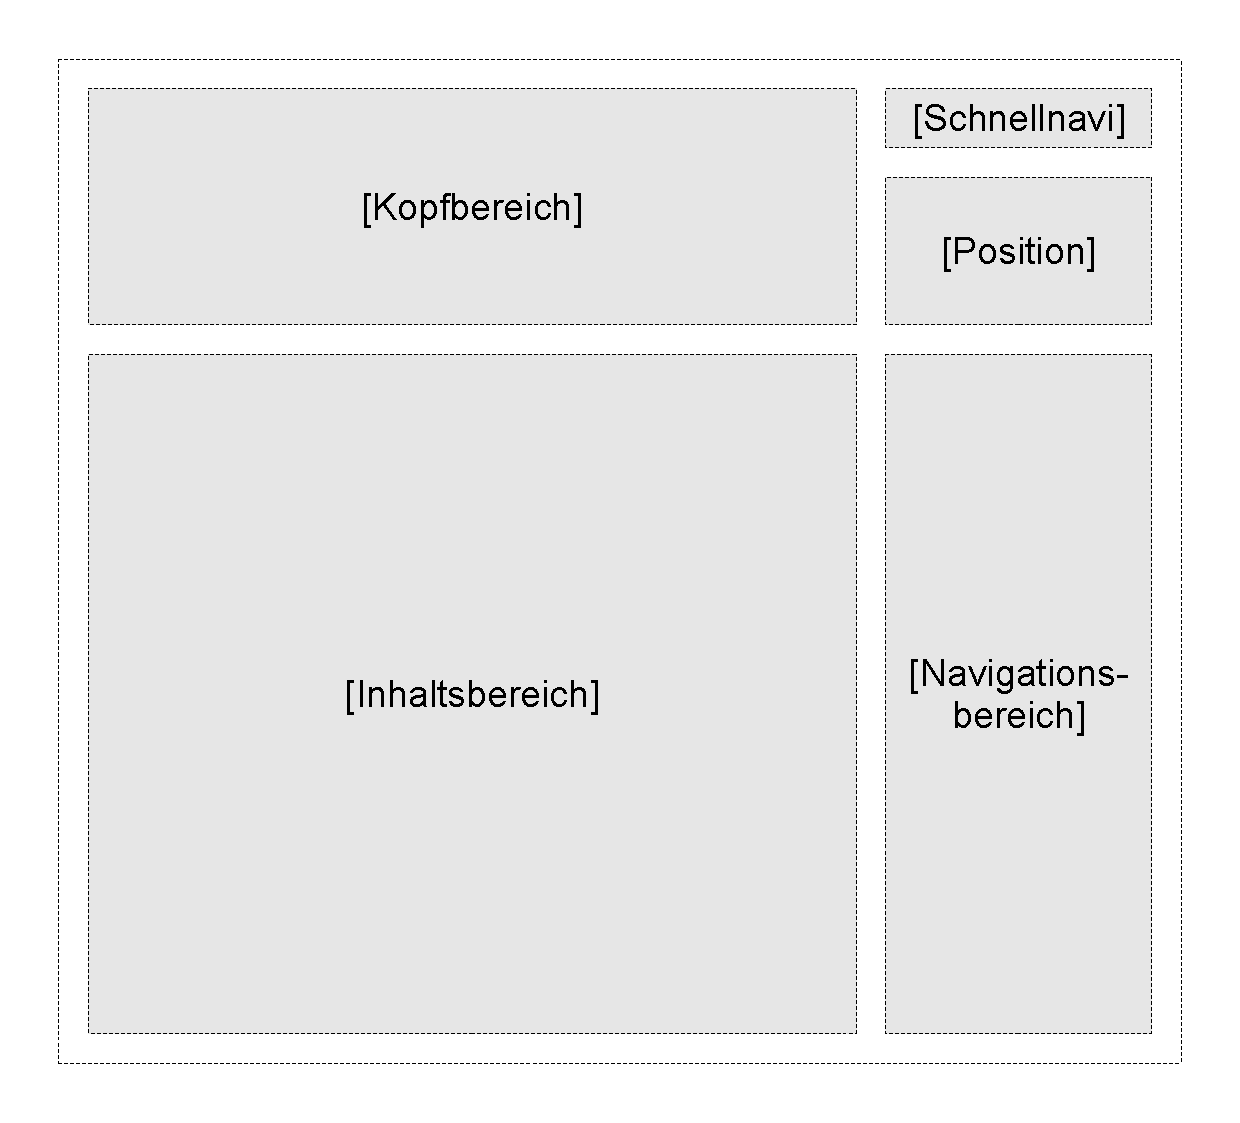
\includegraphics[width=0.5\textwidth]{layout}\\
  \caption{Seitenlayout}
  \label{fig:layout}
\end{figure}


%
%
%
\section*{Hauptseite}
\label{sec:main-page}

Die Hauptseite zeigt folgende Inhalte
\begin{description}
  \item[Textbereich] \texttt{main-page-content.html} Willkommens- und Beschreibungstext der Anwendung. Der Besucher bzw. der Benutzer wird über die Ziele der Anwendung informiert und erhält Anweisungen zum weiteren Vorgehen.
  \item[Wo bin ich] Es erscheinen folgende Zeilen \emph{\\Du bist hier \\Hauptseite}
  \item[Navigation] Zeigt die 5 zuletzt verwendeten Module als einzelne Links an. Alle Module sind zusätzlich über ein Dropdownmenü erreichbar.
	
\end{description}

\begin{figure}[!ht]
  \centering
  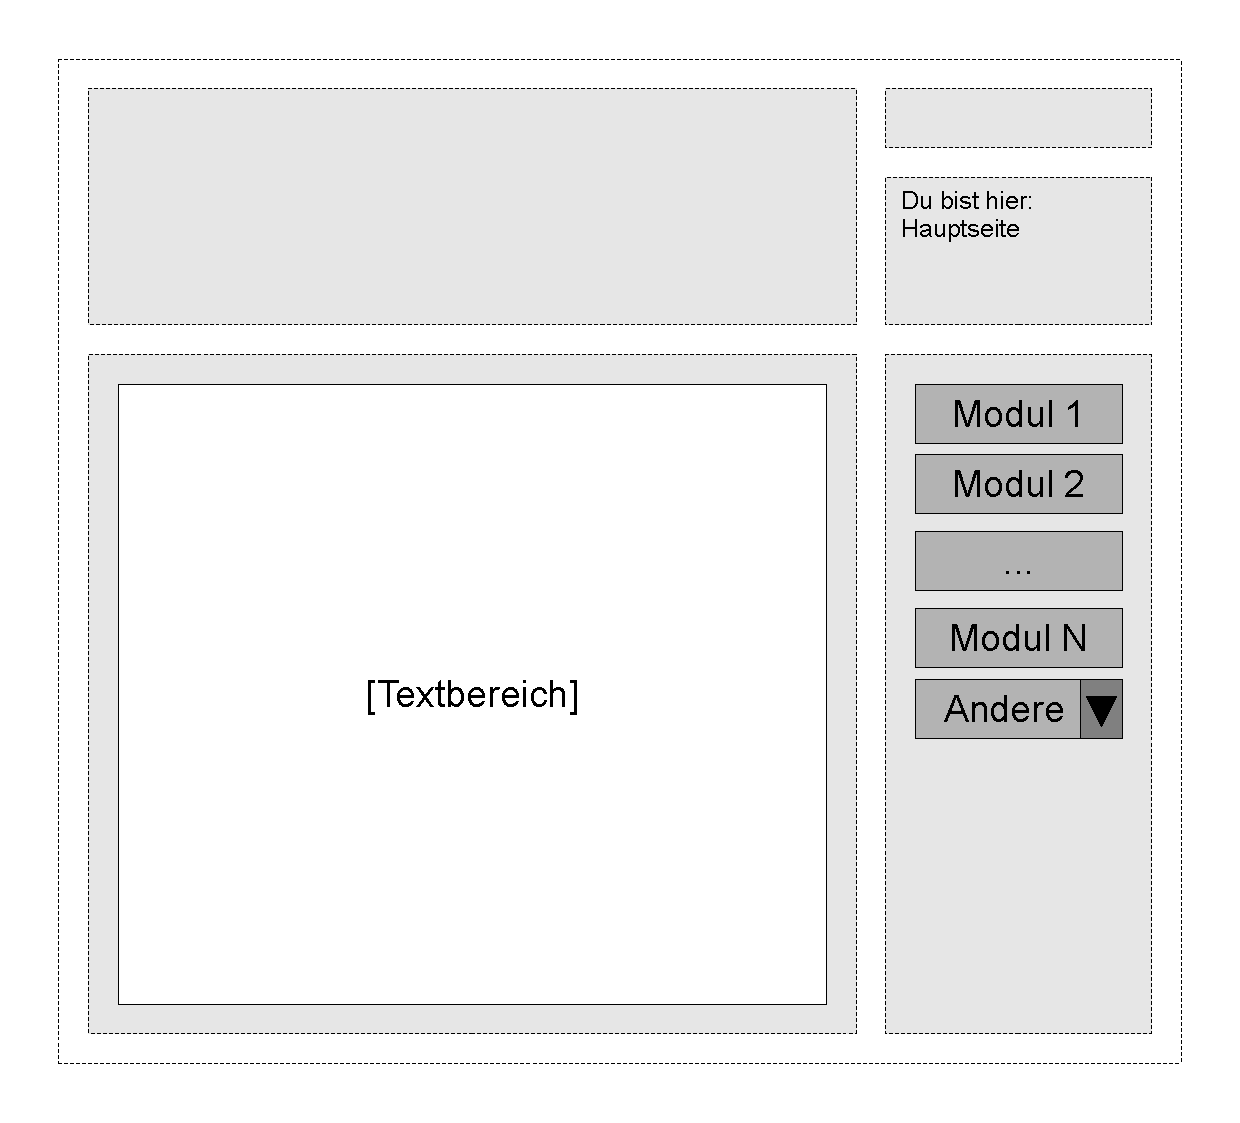
\includegraphics[width=0.5\textwidth]{main-page}\\
  \caption{Hauptseite}
  \label{fig:main-page}
\end{figure}



%
%
%
\section*{Profilseite}
\label{sec:profile-page}

\begin{description}
  \item[Facebookbereich] Optionen zur Facebookverknüpfung. Diese sind bisher undefiniert.
  \item[Statistikbereich] Zeigt die ausgewählte Statistik an. Statistiken sind im Drehbuch der einzelnen Module definiert.
  \item[Wo bin ich] \emph{\\Du bist hier:\\Profilbereich\\Benutzername}
  \item[Navigationsbereich] Zeigt die 5 letzten Module, die eine Statistik über den Benutzer erfasst haben, als einzelne 	Links an. Alle Module mit einer erfassten benutzerstatistik sind zusätzlich über ein Dropdownmenü 	erreichbar.
\end{description}


\begin{figure}[!ht]
  \centering
  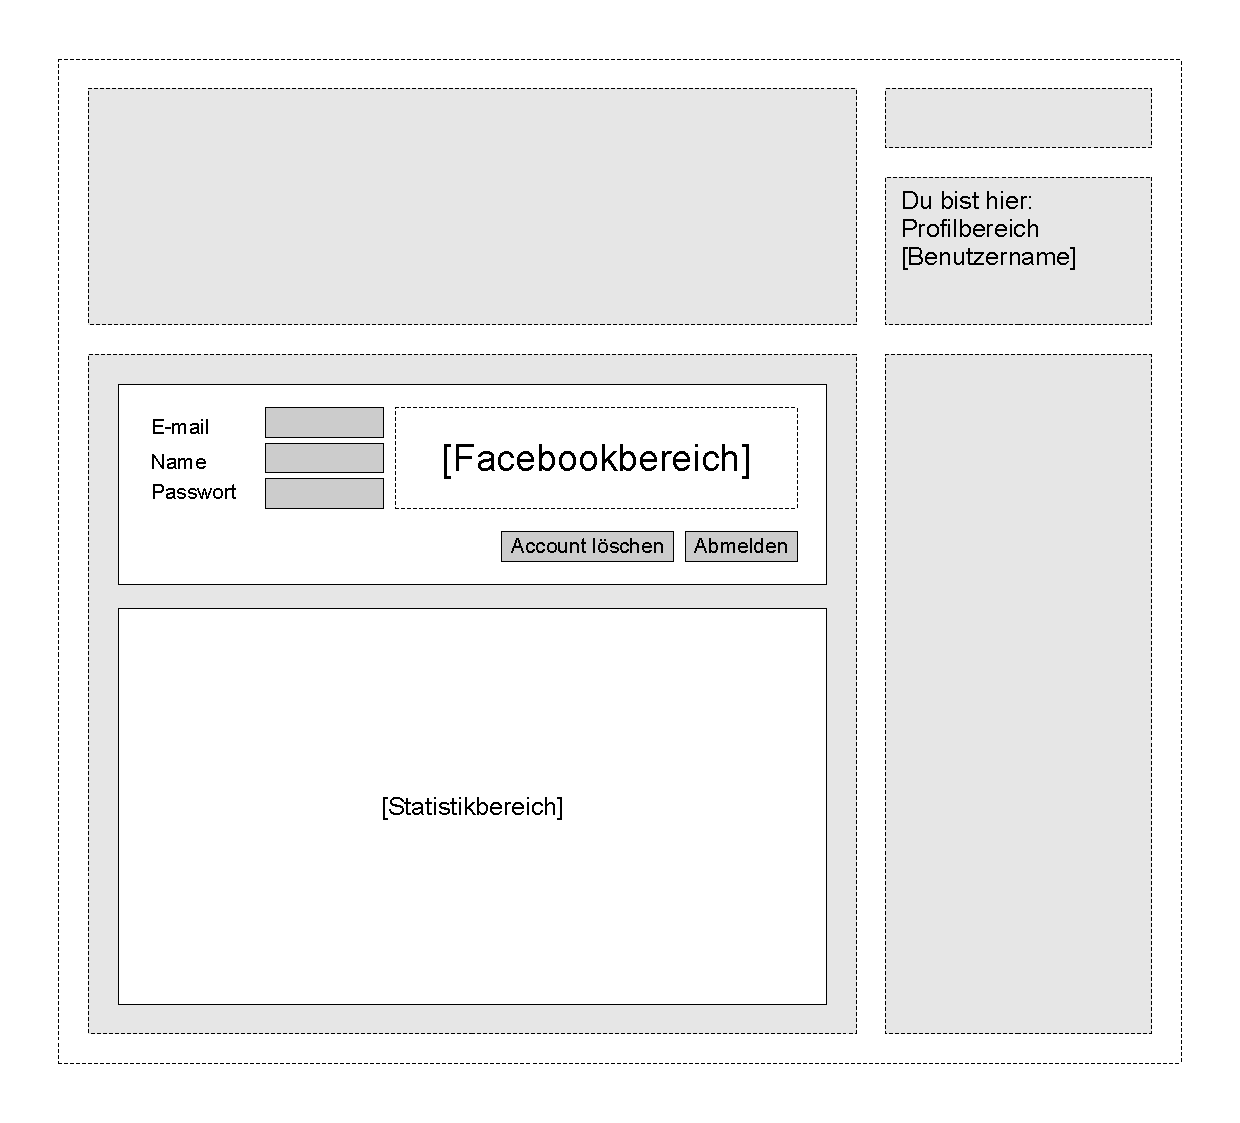
\includegraphics[width=0.5\textwidth]{profile-page}\\
  \caption{Profilseite}
  \label{fig:profile-page}
\end{figure}



%
%
%
\section*{Modulhauptseite}
\label{sec:module-main-page}

\begin{figure}[!ht]
  \centering
  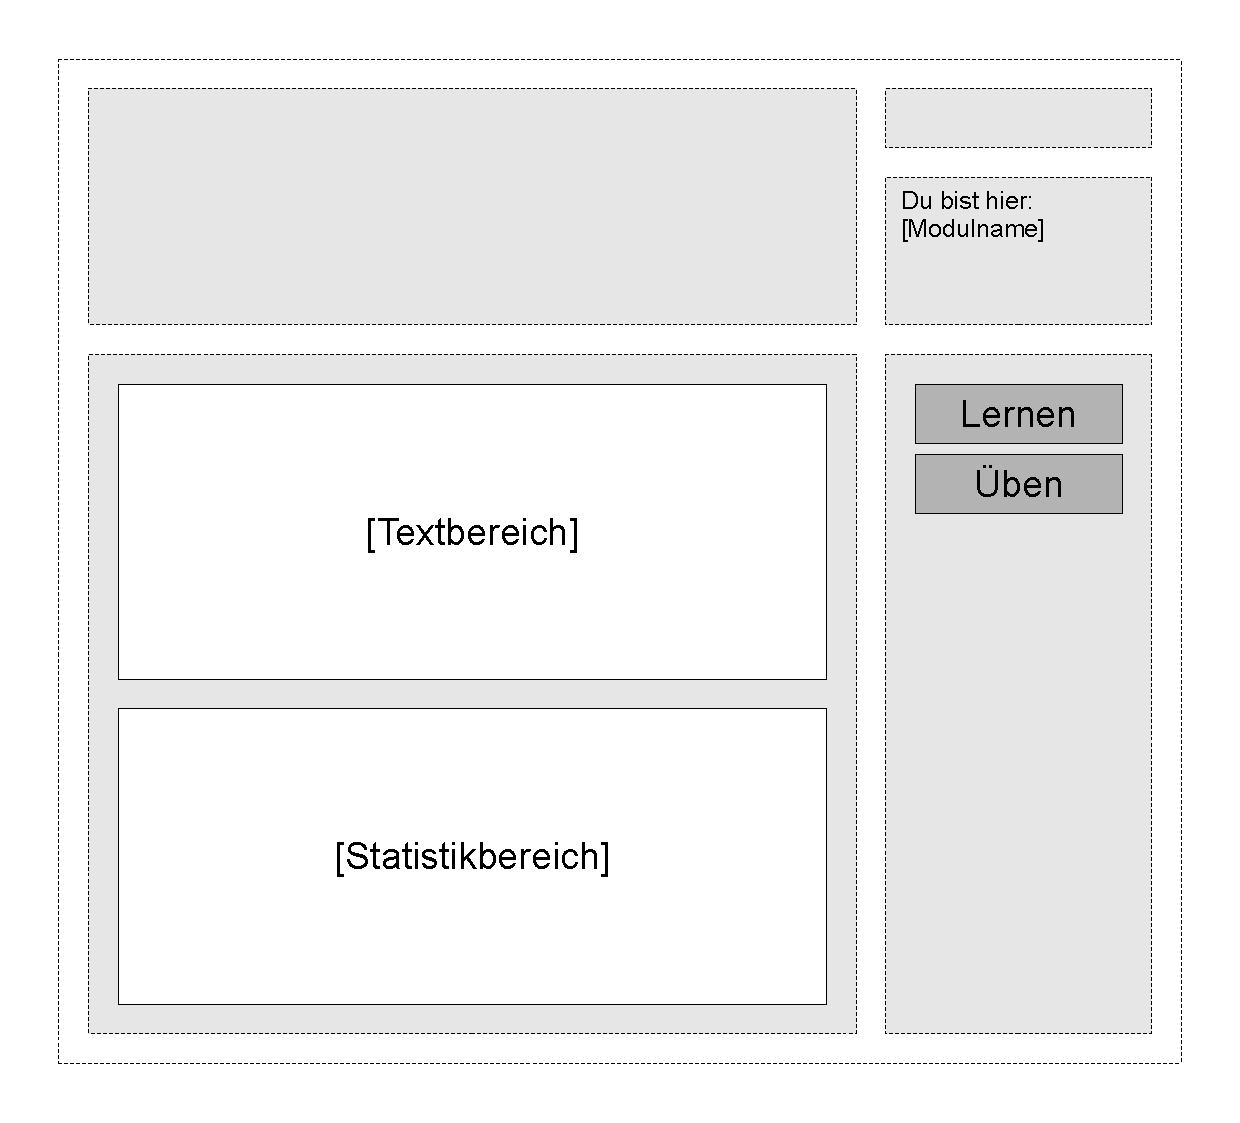
\includegraphics[width=0.5\textwidth]{module-main-page}\\
  \caption{Modulhauptseite}
  \label{fig:module-main-page}
\end{figure}

\begin{description}
  \item[Textbereich] Beschreibt das Modul und dessen Lernziele.
  \item[Statistikbereich] 
    Falls das Modul Statistiken des Benutzers aufgezeichnet hat, so tauchen diese hier auf. Mögliche Statistiken sind:
    \begin{itemize}
      \item Anzahl falscher Antworten.
      \item Anzahl gelernter Vokabeln.
      \item etc
    \end{itemize}
  \item[Wo bin ich] 
    \emph{\\Du bist hier:\\Profilbereich\\Benutzername}
  \item[Navigationsbereich] Enthält folgende Navigationsknöpfe \\
   \begin{description}
    \item[Lernen] Verlinkt auf den Lernbereich des Moduls.
    \item[Üben] Verlinkt auf den Trainingsbereich des Moduls.
   \end{description}
\end{description}

%
%
%
\section*{Modul- Lernseite}
\label{sec:hauptseite}

\begin{description}
  \item[Seiteninhaltsbereich] Der Inhalt eines Moduls ist individuell gestaltbar und kann folgende Elemente enthalten:
  \begin{itemize}
    \item Texte
    \item Grafiken
    \item Videos
    \item Sprechertexte
    \item Externe / interne Links
  \end{itemize}
  
  \item[Wo bin ich] \emph{\\Du bist hier:\\<Modulname>\\<Lernen> - <Aktuelle Seite>}
  \item[Navigationsbereich] Zeigt alle Seiten des Lernbereichs in Form einer Baumstruktur an. Sollte die aktuelle Seite mit einer Trainingseinheit verknüpft sein, so wird neben dem Seitenlink ein Trainingsicon angezeigt %\texttt{training_icon.png} 
  der auf die Trainingseinheit verlinkt.
  
\end{description}

\begin{figure}[!ht]
  \centering
  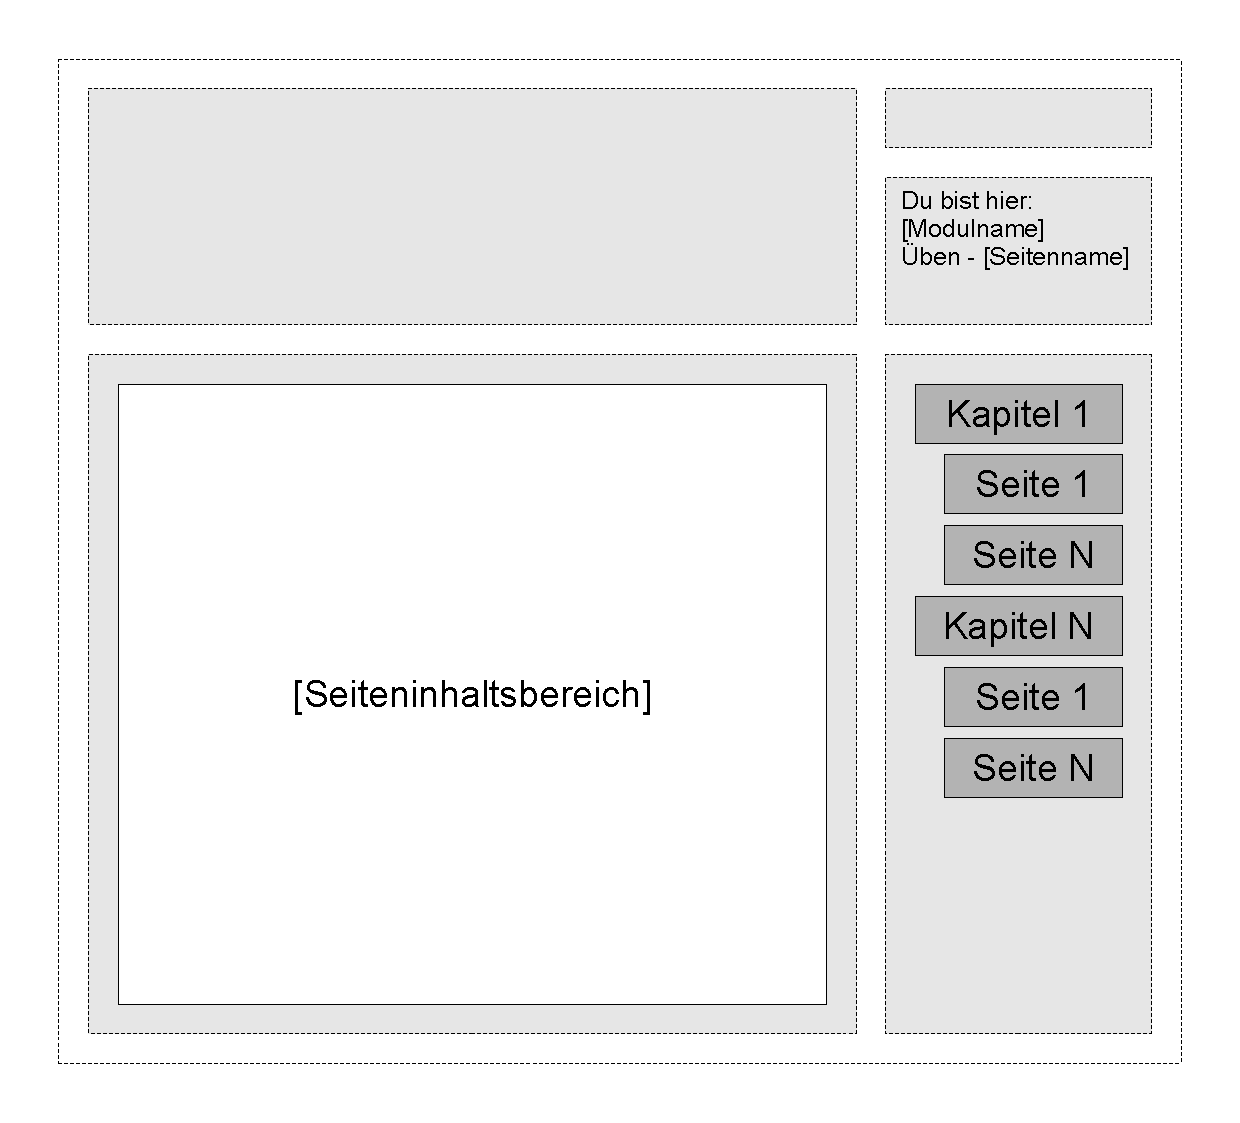
\includegraphics[width=0.5\textwidth]{module-learn-page}\\
  \caption{Modul- Lernseite}
  \label{fig:module-main-page}
\end{figure}

%
%
%
\section*{Modul- Übungsseite}
\label{sec:module-training-page}

\begin{description}
  \item[Aufgabenbereich] Art und Aussehen von Aufgaben sind in den jeweiligen Kapiteln des Drehbuchs beschrieben. Hier sollten zumindest die folgenden Elemente auftauchen:
  \begin{itemize}
    \item Aufgabenstellung
    \item Eingabefelder zur Lösung
    \item evtl. ein Aufgabe lösen Link.
  \end{itemize}
  \item[Wo bin ich] \emph{\\Du bist hier:\\<Modulname>\\<Üben> - <Aktuelles Training>}
  \item[Navigationsbereich] Zeigt alle Trainingseinheiten des Trainingsbereichs in einer Liste an. Sollte die aktuelle Seite mit einer Lernseite verknüpft sein, so wird neben dem Link ein Lernicon angezeigt 
  %\texttt{learning_icon.png} 
  der auf die Lernseite verlinkt.
\end{description}

\begin{figure}[!ht]
  \centering
  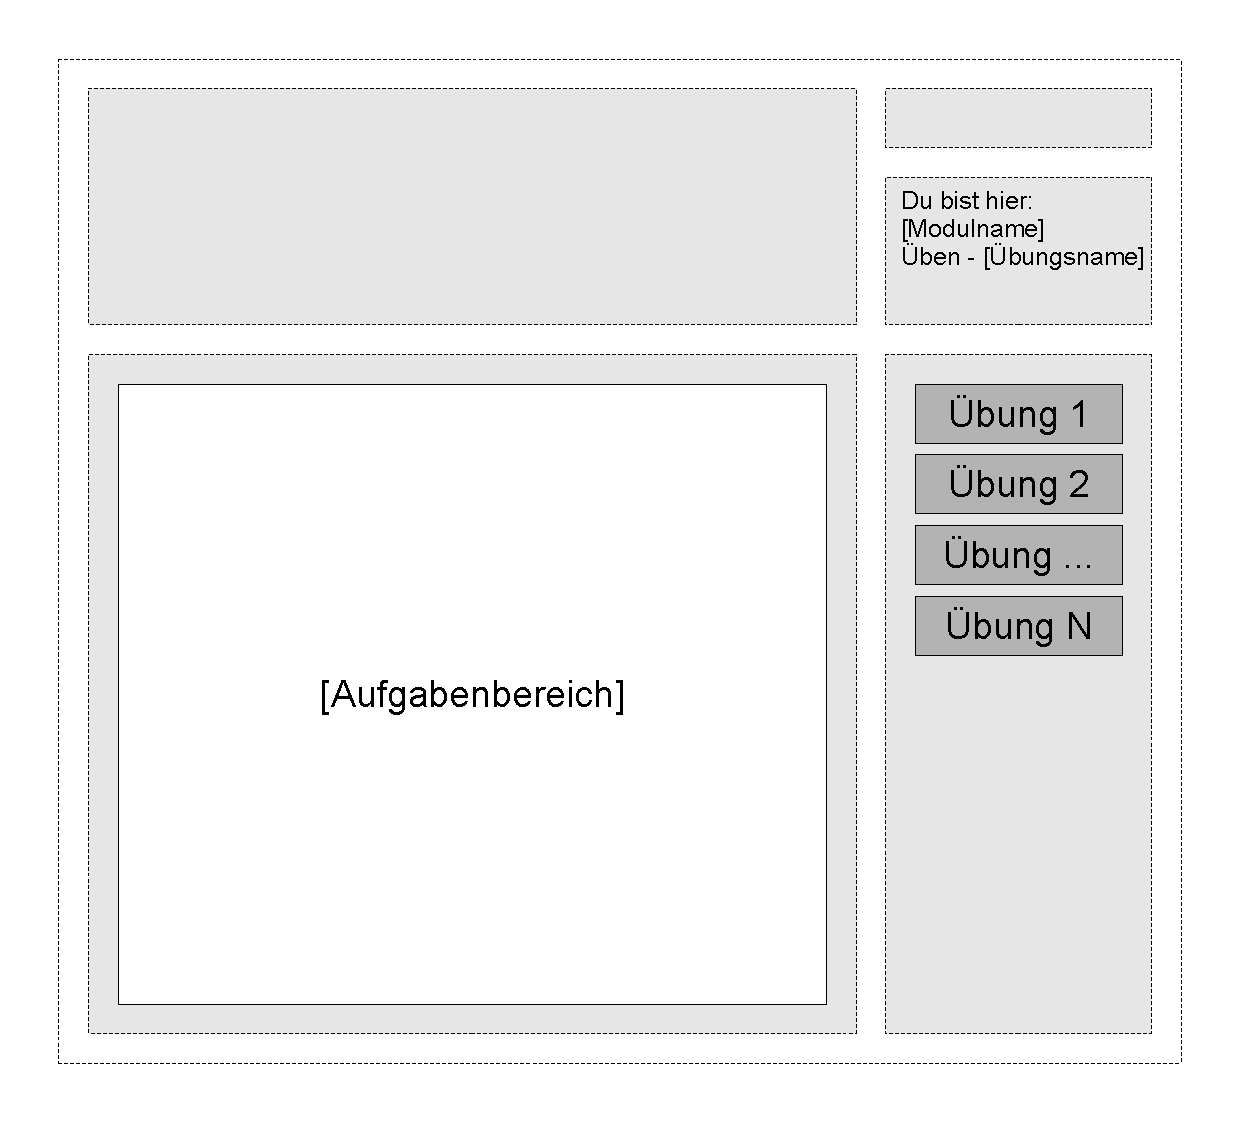
\includegraphics[width=0.5\textwidth]{module-training-page}\\
  \caption{Modul- Übungsseite}
  \label{fig:module-training-page}
\end{figure}


\endinput 
